%% Figure: MMS extra-detection topology classification scatter
%% Data source: data/output/heliosphere/ablations/mms_fte_case_study.json
%% Experiment: E-266 (MMS SITL-labeled eval)  |  Claims: registration pending
%%
%% 86 CD fires that do NOT match any FPI-catalog FTE event.
%% Axes: compressiveness = delta_B/|B| (5-min centered window)
%%        rotation_deg   = B-vector rotation angle (degrees)
%% Threshold lines: compressiveness=0.30, rotation=15 deg
%% Classification quadrants:
%%   Combined (NE):     both rotation>=15 AND compression>=0.30  => 71 (82.6%)
%%   Rotational (NW):   rotation>=15, compression<0.30           =>  4 ( 4.7%)
%%   Compressive (SE):  rotation<15,  compression>=0.30          => 11 (12.8%)
%%   Weak (SW):         both below threshold                     =>  0 ( 0.0%)
%% Topology-positive (combined + rotational): 75/86 = 87.2%
\documentclass[tikz,border=4pt]{standalone}
\usepackage{pgfplots}
\pgfplotsset{compat=1.18}
\usepackage{xcolor}

\definecolor{OIblue}{RGB}{0,114,178}
\definecolor{OIorange}{RGB}{230,159,0}
\definecolor{OIgreen}{RGB}{0,158,115}
\definecolor{OIgray}{RGB}{153,153,153}

\begin{document}
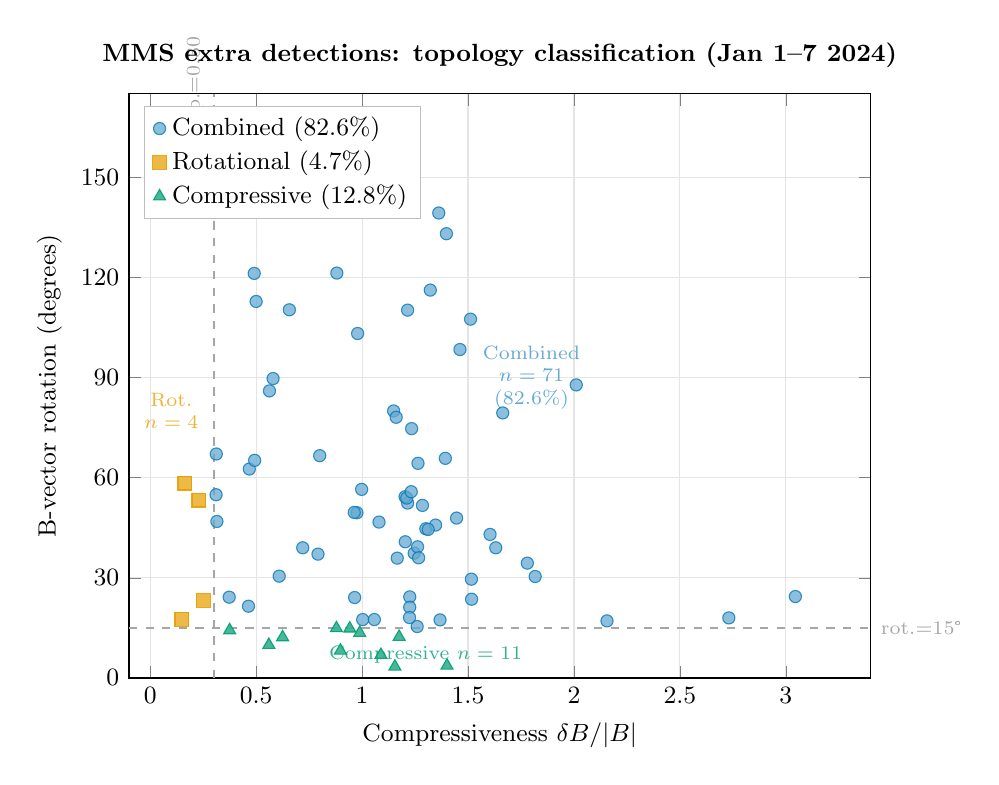
\begin{tikzpicture}
\begin{axis}[
    width=11cm,
    height=9cm,
    xlabel={Compressiveness $\delta B / |B|$},
    ylabel={B-vector rotation (degrees)},
    xmin=-0.1, xmax=3.4,
    ymin=0,    ymax=175,
    xtick={0,0.5,1.0,1.5,2.0,2.5,3.0},
    ytick={0,30,60,90,120,150},
    xticklabel style={font=\small},
    yticklabel style={font=\small},
    xlabel style={font=\small},
    ylabel style={font=\small},
    legend style={at={(0.02,0.98)}, anchor=north west, font=\small,
                  draw=gray!50, fill=white},
    legend cell align=left,
    grid=major,
    grid style={gray!20},
    title style={font=\small\bfseries},
    title={MMS extra detections: topology classification (Jan 1--7 2024)},
    clip=false,
]

%% Threshold lines
\draw[dashed, thick, gray!70]
    (axis cs:0.30, 0) -- (axis cs:0.30, 175)
    node[above, font=\scriptsize, text=gray!70, rotate=90, anchor=south] {comp.=0.30};
\draw[dashed, thick, gray!70]
    (axis cs:-0.1, 15) -- (axis cs:3.4, 15)
    node[right, font=\scriptsize, text=gray!70] {rot.=15\textdegree};

%% Quadrant labels (subtle background annotation)
\node[font=\scriptsize, text=OIblue!60, align=center] at (axis cs:1.8,90) {Combined\\$n=71$\\(82.6\%)};
\node[font=\scriptsize, text=OIorange!80, align=center] at (axis cs:0.10,80) {Rot.\\$n=4$};
\node[font=\scriptsize, text=OIgreen!80, align=center] at (axis cs:1.3,7) {Compressive  $n=11$};

%% Combined: 71 points
\addplot[only marks, mark=*, mark size=2.2pt, color=OIblue, fill=OIblue!60,
         opacity=0.75] coordinates {
  (2.731,18.0)
  (3.045,24.4)
  (0.979,103.2)
  (1.204,40.8)
  (1.003,17.5)
  (0.373,24.2)
  (0.563,86.0)
  (0.580,89.7)
  (0.657,110.3)
  (1.246,37.4)
  (1.664,79.4)
  (1.512,107.5)
  (1.393,65.8)
  (0.881,121.3)
  (1.215,110.2)
  (0.998,56.5)
  (0.800,66.6)
  (1.264,64.3)
  (1.262,39.3)
  (1.080,46.7)
  (1.301,44.7)
  (1.604,43.0)
  (0.311,54.9)
  (0.609,30.5)
  (0.691,157.1)
  (0.638,160.0)
  (0.491,121.2)
  (0.500,112.8)
  (0.468,62.6)
  (0.464,21.5)
  (1.516,29.6)
  (0.976,49.5)
  (1.215,52.4)
  (1.203,54.3)
  (1.780,34.4)
  (1.211,53.9)
  (1.631,39.0)
  (2.011,87.8)
  (1.347,45.8)
  (1.225,24.3)
  (1.232,55.8)
  (1.047,149.3)
  (1.362,139.3)
  (1.285,51.7)
  (1.267,36.0)
  (1.149,80.0)
  (1.166,35.9)
  (0.965,24.1)
  (1.260,15.4)
  (1.225,21.2)
  (1.234,74.7)
  (1.162,154.1)
  (1.208,156.1)
  (1.398,133.1)
  (1.224,18.1)
  (1.368,17.4)
  (1.446,47.9)
  (1.312,44.5)
  (1.058,17.5)
  (0.963,49.6)
  (0.720,39.0)
  (1.817,30.4)
  (2.156,17.1)
  (0.792,37.1)
  (0.493,65.2)
  (0.312,67.1)
  (0.315,46.9)
  (1.161,78.1)
  (1.322,116.2)
  (1.517,23.6)
  (1.462,98.4)
};
\addlegendentry{Combined (82.6\%)}

%% Rotational: 4 points
\addplot[only marks, mark=square*, mark size=2.5pt, color=OIorange,
         fill=OIorange!80, opacity=0.90] coordinates {
  (0.230,53.3)
  (0.164,58.4)
  (0.251,23.2)
  (0.150,17.6)
};
\addlegendentry{Rotational (4.7\%)}

%% Compressive: 11 points
\addplot[only marks, mark=triangle*, mark size=2.5pt, color=OIgreen,
         fill=OIgreen!80, opacity=0.90] coordinates {
  (0.375,14.3)
  (0.898,8.2)
  (0.989,13.5)
  (1.089,6.9)
  (1.155,3.4)
  (1.401,3.7)
  (1.175,12.3)
  (0.625,12.2)
  (0.560,9.9)
  (0.942,14.8)
  (0.879,14.9)
};
\addlegendentry{Compressive (12.8\%)}

\end{axis}
\end{tikzpicture}
\end{document}
